\documentclass[journal,12pt,twocolumn]{IEEEtran}
\usepackage{listings}
\usepackage{ragged2e}
\usepackage[utf8]{inputenc}
\usepackage{subcaption}
\usepackage{tikz}
\usepackage[export]{adjustbox}
\usepackage{tkz-euclide} % loads  TikZ and tkz-base
%\usetkzobj{all}
\usetikzlibrary{calc,math}
\usepackage{amsmath}
\lstset{
%language=C,
frame=single, 
breaklines=true,
columns=fullflexible
}
\usepackage{float}
\renewcommand{\vec}[1]{\mathbf{#1}}
\newcommand\norm[1]{\left\lVert#1\right\rVert}
\title{Document on Question 28 Exercise(8.1)}
\author{Pothukuchi Siddhartha}

\begin{document}

\maketitle
\begin{abstract}
This a simple document explaining a question about the concept of similar triangles.
\end{abstract}
Download all python codes from 
%


\begin{lstlisting}
svn co https://github.com/SiddharthPh/Summer2020/trunk/geometry/codes
\end{lstlisting}
%

\section*{\textbf{Question}}
In right triangle ABC, right angled at C, M is
the mid-point of hypotenuse AB. C is joined to
M and produced to a point D such that DM =
CM. Point D is joined to point B. Show that:
\newline
a)$\triangle  AMC  \cong   \triangle  BMD $
\newline
b)$\triangle DBC $ is a right angle.
\newline
c)$\triangle  DBC  \cong  \triangle  ABC $
\newline
d)CM = $\frac{1}{2}$ AB

\section*{\textbf{Construction}}
\renewcommand{\theequation}{\theenumi}
\begin{enumerate}[label=\thesection.\arabic*.,ref=\thesection.\theenumi]
\numberwithin{equation}{enumi}
\item The figure for A triangle obtained in the question looks like Fig. \ref{fig:tri_right_angle}.
with angles $\phase{ A},\phase{ C}$ and $\phase{ B}$ and sides $a, b$ and $c$.  The unique feature of this triangle is $\phase{ C}$ which is defined to be $90\degree$.


%\renewcommand{\thefigure}{\theenumi.\arabic{figure}}
\begin{figure}[!ht]
\centering
\resizebox{\columnwidth}{!}{

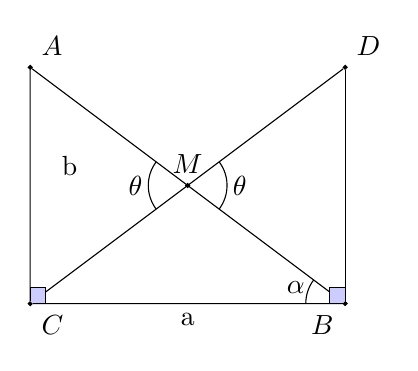
\begin{tikzpicture}
[scale=1,>=stealth,point/.style={draw,circle,fill = black,inner sep=0.5pt},]

%Triangle sides
\def\a{4}
\def\b{3}
\def\c{sqrt(\a^2+\c^2)}



%Labeling points
\node (A) at (0,\b)[point,label=above right:$A$] {};
\node (B) at (\a, 0)[point,label=below left:$B$] {};
\node (C) at (0, 0)[point,label=below right:$C$] {};
\node (M) at (\a*0.5,\b*0.5)[point,label=above:$M$] {};
\node (D) at (\a,\b)[point,label=above right:$D$] {};


%Drawing triangle ABC
\draw (A) -- node[left] {$\textrm{}$} (B) -- node[below] {$\textrm{a}$} (C) -- node[above,xshift=5mm] {$\textrm{b}$} (A);

%Joining CD
\draw (C)--(D);
%Joining BD
\draw (B)--(D);

%Drawing and marking angles
\tkzMarkAngle[fill=orange!40,size=0.5cm,mark=](A,M,C)
\tkzMarkAngle[fill=orange!40,size=0.5cm,mark=](B,M,D)
\tkzMarkAngle[fill=green!40,size=0.5cm,mark=](A,B,C)
\tkzMarkRightAngle[fill=blue!20,size=.2](A,C,B)
\tkzMarkRightAngle[fill=blue!20,size=.2](D,B,C)
\tkzLabelAngle[pos=0.65](A,M,C){$\theta$}
\tkzLabelAngle[pos=0.65](B,M,D){$\theta$}
\tkzLabelAngle[pos=0.65](A,B,C){$\alpha$}


\end{tikzpicture}
}
\caption{Right Angled Triangle by Latex-Tikz}
\label{fig:tri_right_angle}	
\end{figure}
%
%
%\renewcommand{\thefigure}{\theenumi}
%
\item List the design parameters for construction
\label{const:table1}
\\
\solution See Table. \ref{table:table1}. 
%
\begin{table}[ht!]
\centering
%\begin{tabular}{ |p{3cm}|p{3cm}|  }
%\hline
% \multicolumn{2}{|c|}{Initial Input Values.} \\
%\hline
%a & 4\\
%\hline
%b & 3\\
%\hline
%$\phase{(ACB)$ & $90^{\circ}$ \\
%\hline
%\end{tabular}
%%%%%%%%%%%%%%%%%%%%%%%%%%%%%%%%%%%%%%%%%%%%%%%%%%%%%%%%%%%%%%%%%%%%%%
%%                                                                  %%
%%  This is the header of a LaTeX2e file exported from Gnumeric.    %%
%%                                                                  %%
%%  This file can be compiled as it stands or included in another   %%
%%  LaTeX document. The table is based on the longtable package so  %%
%%  the longtable options (headers, footers...) can be set in the   %%
%%  preamble section below (see PRAMBLE).                           %%
%%                                                                  %%
%%  To include the file in another, the following two lines must be %%
%%  in the including file:                                          %%
%%        \def\inputGnumericTable{}                                 %%
%%  at the beginning of the file and:                               %%
%%        \input{name-of-this-file.tex}                             %%
%%  where the table is to be placed. Note also that the including   %%
%%  file must use the following packages for the table to be        %%
%%  rendered correctly:                                             %%
%%    \usepackage[latin1]{inputenc}                                 %%
%%    \usepackage{color}                                            %%
%%    \usepackage{array}                                            %%
%%    \usepackage{longtable}                                        %%
%%    \usepackage{calc}                                             %%
%%    \usepackage{multirow}                                         %%
%%    \usepackage{hhline}                                           %%
%%    \usepackage{ifthen}                                           %%
%%  optionally (for landscape tables embedded in another document): %%
%%    \usepackage{lscape}                                           %%
%%                                                                  %%
%%%%%%%%%%%%%%%%%%%%%%%%%%%%%%%%%%%%%%%%%%%%%%%%%%%%%%%%%%%%%%%%%%%%%%



%%  This section checks if we are begin input into another file or  %%
%%  the file will be compiled alone. First use a macro taken from   %%
%%  the TeXbook ex 7.7 (suggestion of Han-Wen Nienhuys).            %%
\def\ifundefined#1{\expandafter\ifx\csname#1\endcsname\relax}


%%  Check for the \def token for inputed files. If it is not        %%
%%  defined, the file will be processed as a standalone and the     %%
%%  preamble will be used.                                          %%
\ifundefined{inputGnumericTable}

%%  We must be able to close or not the document at the end.        %%
	\def\gnumericTableEnd{\end{document}}


%%%%%%%%%%%%%%%%%%%%%%%%%%%%%%%%%%%%%%%%%%%%%%%%%%%%%%%%%%%%%%%%%%%%%%
%%                                                                  %%
%%  This is the PREAMBLE. Change these values to get the right      %%
%%  paper size and other niceties.                                  %%
%%                                                                  %%
%%%%%%%%%%%%%%%%%%%%%%%%%%%%%%%%%%%%%%%%%%%%%%%%%%%%%%%%%%%%%%%%%%%%%%

	\documentclass[12pt%
			  %,landscape%
                    ]{report}
       \usepackage[latin1]{inputenc}
       \usepackage{fullpage}
       \usepackage{color}
       \usepackage{array}
       \usepackage{longtable}
       \usepackage{calc}
       \usepackage{multirow}
       \usepackage{hhline}
       \usepackage{ifthen}
        \usepackage[cmex10]{amsmath}
       \newcommand{\myvec}[1]{\ensuremath{\begin{pmatrix}#1\end{pmatrix}}}

	\begin{document}


%%  End of the preamble for the standalone. The next section is for %%
%%  documents which are included into other LaTeX2e files.          %%
\else

%%  We are not a stand alone document. For a regular table, we will %%
%%  have no preamble and only define the closing to mean nothing.   %%
    \def\gnumericTableEnd{}

%%  If we want landscape mode in an embedded document, comment out  %%
%%  the line above and uncomment the two below. The table will      %%
%%  begin on a new page and run in landscape mode.                  %%
%       \def\gnumericTableEnd{\end{landscape}}
%       \begin{landscape}


%%  End of the else clause for this file being \input.              %%
\fi

%%%%%%%%%%%%%%%%%%%%%%%%%%%%%%%%%%%%%%%%%%%%%%%%%%%%%%%%%%%%%%%%%%%%%%
%%                                                                  %%
%%  The rest is the gnumeric table, except for the closing          %%
%%  statement. Changes below will alter the table's appearance.     %%
%%                                                                  %%
%%%%%%%%%%%%%%%%%%%%%%%%%%%%%%%%%%%%%%%%%%%%%%%%%%%%%%%%%%%%%%%%%%%%%%

\providecommand{\gnumericmathit}[1]{#1} 
%%  Uncomment the next line if you would like your numbers to be in %%
%%  italics if they are italizised in the gnumeric table.           %%
%\renewcommand{\gnumericmathit}[1]{\mathit{#1}}
\providecommand{\gnumericPB}[1]%
{\let\gnumericTemp=\\#1\let\\=\gnumericTemp\hspace{0pt}}
 \ifundefined{gnumericTableWidthDefined}
        \newlength{\gnumericTableWidth}
        \newlength{\gnumericTableWidthComplete}
        \newlength{\gnumericMultiRowLength}
        \global\def\gnumericTableWidthDefined{}
 \fi
%% The following setting protects this code from babel shorthands.  %%
 \ifthenelse{\isundefined{\languageshorthands}}{}{\languageshorthands{english}}
%%  The default table format retains the relative column widths of  %%
%%  gnumeric. They can easily be changed to c, r or l. In that case %%
%%  you may want to comment out the next line and uncomment the one %%
%%  thereafter                                                      %%
\providecommand\gnumbox{\makebox[0pt]}
%%\providecommand\gnumbox[1][]{\makebox}

%% to adjust positions in multirow situations                       %%
\setlength{\bigstrutjot}{\jot}
\setlength{\extrarowheight}{\doublerulesep}

%%  The \setlongtables command keeps column widths the same across  %%
%%  pages. Simply comment out next line for varying column widths.  %%
\setlongtables

\setlength\gnumericTableWidth{%
	71pt+%
	95pt+%
0pt}
\def\gumericNumCols{2}
\setlength\gnumericTableWidthComplete{\gnumericTableWidth+%
         \tabcolsep*\gumericNumCols*2+\arrayrulewidth*\gumericNumCols}
\ifthenelse{\lengthtest{\gnumericTableWidthComplete > \linewidth}}%
         {\def\gnumericScale{\ratio{\linewidth-%
                        \tabcolsep*\gumericNumCols*2-%
                        \arrayrulewidth*\gumericNumCols}%
{\gnumericTableWidth}}}%
{\def\gnumericScale{1}}

%%%%%%%%%%%%%%%%%%%%%%%%%%%%%%%%%%%%%%%%%%%%%%%%%%%%%%%%%%%%%%%%%%%%%%
%%                                                                  %%
%% The following are the widths of the various columns. We are      %%
%% defining them here because then they are easier to change.       %%
%% Depending on the cell formats we may use them more than once.    %%
%%                                                                  %%
%%%%%%%%%%%%%%%%%%%%%%%%%%%%%%%%%%%%%%%%%%%%%%%%%%%%%%%%%%%%%%%%%%%%%%

\ifthenelse{\isundefined{\gnumericColA}}{\newlength{\gnumericColA}}{}\settowidth{\gnumericColA}{\begin{tabular}{@{}p{71pt*\gnumericScale}@{}}x\end{tabular}}
\ifthenelse{\isundefined{\gnumericColB}}{\newlength{\gnumericColB}}{}\settowidth{\gnumericColB}{\begin{tabular}{@{}p{95pt*\gnumericScale}@{}}x\end{tabular}}

\begin{tabular}[c]{%
	b{\gnumericColA}%
	b{\gnumericColB}%
	}

%%%%%%%%%%%%%%%%%%%%%%%%%%%%%%%%%%%%%%%%%%%%%%%%%%%%%%%%%%%%%%%%%%%%%%
%%  The longtable options. (Caption, headers... see Goosens, p.124) %%
%	\caption{The Table Caption.}             \\	%
% \hline	% Across the top of the table.
%%  The rest of these options are table rows which are placed on    %%
%%  the first, last or every page. Use \multicolumn if you want.    %%

%%  Header for the first page.                                      %%
%	\multicolumn{2}{c}{The First Header} \\ \hline 
%	\multicolumn{1}{c}{colTag}	%Column 1
%	&\multicolumn{1}{c}{colTag}	\\ \hline %Last column
%	\endfirsthead

%%  The running header definition.                                  %%
%	\hline
%	\multicolumn{2}{l}{\ldots\small\slshape continued} \\ \hline
%	\multicolumn{1}{c}{colTag}	%Column 1
%	&\multicolumn{1}{c}{colTag}	\\ \hline %Last column
%	\endhead

%%  The running footer definition.                                  %%
%	\hline
%	\multicolumn{2}{r}{\small\slshape continued\ldots} \\
%	\endfoot

%%  The ending footer definition.                                   %%
%	\multicolumn{2}{c}{That's all folks} \\ \hline 
%	\endlastfoot
%%%%%%%%%%%%%%%%%%%%%%%%%%%%%%%%%%%%%%%%%%%%%%%%%%%%%%%%%%%%%%%%%%%%%%

\hhline{|--}
	 \multicolumn{2}{|p{	\gnumericColA+%
	\gnumericColB+%
	\tabcolsep*2*1}|}%
	{\gnumericPB{\centering}\gnumbox{Input values}}
\\
\hhline{|-|-|}
	 \multicolumn{1}{|p{\gnumericColA}|}%
	{\gnumericPB{\centering}\gnumbox{Parameters}}
	&\multicolumn{1}{p{\gnumericColB}|}%
	{\gnumericPB{\centering}\gnumbox{Values}}
\\
\hhline{|--|}
	 \multicolumn{1}{|p{\gnumericColA}|}%
	{\gnumericPB{\centering}\gnumbox{\textbf{O}}}
	&\multicolumn{1}{p{\gnumericColB}|}%
	{$\myvec{2\\-3}$}
\\
\hhline{|--|}
	 \multicolumn{1}{|p{\gnumericColA}|}%
	{\gnumericPB{\centering}\gnumbox{\textbf{A}}}
	&\multicolumn{1}{p{\gnumericColB}|}%
	{$\myvec{1\\4}$}
\\
\hhline{|-|-|}
\end{tabular}

\ifthenelse{\isundefined{\languageshorthands}}{}{\languageshorthands{\languagename}}
\gnumericTableEnd

\caption{To construct $\triangle ACB$}
\label{table:table1}	
\end{table}

%\item
%	For simplicity, let the greek letter $\alpha = \phase{ B$.  We have the following definitions.
%\begin{equation}
%\label{eq:tri_trig_defs}
%\begin{matrix}
	%\sin \theta = \frac{b}{c} & 	\cos \theta = \frac{a}{c} \\
	%\tan \theta = \frac{c}{a} & \cot \theta = \frac{1}{\tan \theta} \\
	%\csc \theta = \frac{1}{\sin \theta} & \sec \theta = \frac{1}{\cos \theta}
	%\end{equation}
%
\item Find the coordinates of the various points in Fig. \ref{fig:tri_right_angle}
\label{const:tri_right_angle}
\\
%
\solution From the given information, 
%$\triangle ABC$ are 
\begin{align}
\label{eq:constr_a}
\vec{A} &= \myvec{0\\b} 
\\
 \vec{C} &= \myvec{0\\0}, 
\label{eq:constr_c}
\\
\vec{B} &= \myvec{a\\0}
\label{eq:constr_b}
\end{align}
$\because \vec{M}$ is the midpoint of $AB$,
\begin{align}
\vec{M}= \frac{\vec{A}+\vec{B}}{2} = \frac{1}{2}\myvec{a\\b}
\label{eq:constr_m}
\end{align}
%
Also, $\vec{M}$ is given to be the midpoint of $C$.  Hence, 
\begin{align}
\vec{M}&= \frac{\vec{C}+\vec{D}}{2}
\\
\implies \vec{D} &= 2 \vec{M} - \vec{C} = \myvec{a\\b}
\label{eq:constr_d}
\end{align}
%
The values are listed in 
%\item List the  derived values.
%\label{const:table2}
%\\
%\solution See  
Table. \ref{table:table2} 
\begin{table}[ht!]
%\centering
%\begin{tabular}{ |p{3cm}|p{3cm}|  }
%\hline
% \multicolumn{2}{|c|}{Derived Values.} \\
%\hline
%$\vec{M}$ & $$\begin{pmatrix}2\\1.5\end{pmatrix}$$\\						
%\hline
%$\vec{D}$ & $$\begin{pmatrix}4\\3\end{pmatrix} $$\\
%\hline
%%%%%%%%%%%%%%%%%%%%%%%%%%%%%%%%%%%%%%%%%%%%%%%%%%%%%%%%%%%%%%%%%%%%%%
%%                                                                  %%
%%  This is the header of a LaTeX2e file exported from Gnumeric.    %%
%%                                                                  %%
%%  This file can be compiled as it stands or included in another   %%
%%  LaTeX document. The table is based on the longtable package so  %%
%%  the longtable options (headers, footers...) can be set in the   %%
%%  preamble section below (see PRAMBLE).                           %%
%%                                                                  %%
%%  To include the file in another, the following two lines must be %%
%%  in the including file:                                          %%
%%        \def\inputGnumericTable{}                                 %%
%%  at the beginning of the file and:                               %%
%%        \input{name-of-this-file.tex}                             %%
%%  where the table is to be placed. Note also that the including   %%
%%  file must use the following packages for the table to be        %%
%%  rendered correctly:                                             %%
%%    \usepackage[latin1]{inputenc}                                 %%
%%    \usepackage{color}                                            %%
%%    \usepackage{array}                                            %%
%%    \usepackage{longtable}                                        %%
%%    \usepackage{calc}                                             %%
%%    \usepackage{multirow}                                         %%
%%    \usepackage{hhline}                                           %%
%%    \usepackage{ifthen}                                           %%
%%  optionally (for landscape tables embedded in another document): %%
%%    \usepackage{lscape}                                           %%
%%                                                                  %%
%%%%%%%%%%%%%%%%%%%%%%%%%%%%%%%%%%%%%%%%%%%%%%%%%%%%%%%%%%%%%%%%%%%%%%



%%  This section checks if we are begin input into another file or  %%
%%  the file will be compiled alone. First use a macro taken from   %%
%%  the TeXbook ex 7.7 (suggestion of Han-Wen Nienhuys).            %%
\def\ifundefined#1{\expandafter\ifx\csname#1\endcsname\relax}


%%  Check for the \def token for inputed files. If it is not        %%
%%  defined, the file will be processed as a standalone and the     %%
%%  preamble will be used.                                          %%
\ifundefined{inputGnumericTable}

%%  We must be able to close or not the document at the end.        %%
	\def\gnumericTableEnd{\end{document}}


%%%%%%%%%%%%%%%%%%%%%%%%%%%%%%%%%%%%%%%%%%%%%%%%%%%%%%%%%%%%%%%%%%%%%%
%%                                                                  %%
%%  This is the PREAMBLE. Change these values to get the right      %%
%%  paper size and other niceties.                                  %%
%%                                                                  %%
%%%%%%%%%%%%%%%%%%%%%%%%%%%%%%%%%%%%%%%%%%%%%%%%%%%%%%%%%%%%%%%%%%%%%%

	\documentclass[12pt%
			  %,landscape%
                    ]{report}
       \usepackage[latin1]{inputenc}
       \usepackage{fullpage}
       \usepackage{color}
       \usepackage{array}
       \usepackage{longtable}
       \usepackage{calc}
       \usepackage{multirow}
       \usepackage{hhline}
       \usepackage{ifthen}
       \usepackage[cmex10]{amsmath}
       \newcommand{\myvec}[1]{\ensuremath{\begin{pmatrix}#1\end{pmatrix}}}

	\begin{document}


%%  End of the preamble for the standalone. The next section is for %%
%%  documents which are included into other LaTeX2e files.          %%
\else

%%  We are not a stand alone document. For a regular table, we will %%
%%  have no preamble and only define the closing to mean nothing.   %%
    \def\gnumericTableEnd{}

%%  If we want landscape mode in an embedded document, comment out  %%
%%  the line above and uncomment the two below. The table will      %%
%%  begin on a new page and run in landscape mode.                  %%
%       \def\gnumericTableEnd{\end{landscape}}
%       \begin{landscape}


%%  End of the else clause for this file being \input.              %%
\fi

%%%%%%%%%%%%%%%%%%%%%%%%%%%%%%%%%%%%%%%%%%%%%%%%%%%%%%%%%%%%%%%%%%%%%%
%%                                                                  %%
%%  The rest is the gnumeric table, except for the closing          %%
%%  statement. Changes below will alter the table's appearance.     %%
%%                                                                  %%
%%%%%%%%%%%%%%%%%%%%%%%%%%%%%%%%%%%%%%%%%%%%%%%%%%%%%%%%%%%%%%%%%%%%%%

\providecommand{\gnumericmathit}[1]{#1} 
%%  Uncomment the next line if you would like your numbers to be in %%
%%  italics if they are italizised in the gnumeric table.           %%
%\renewcommand{\gnumericmathit}[1]{\mathit{#1}}
\providecommand{\gnumericPB}[1]%
{\let\gnumericTemp=\\#1\let\\=\gnumericTemp\hspace{0pt}}
 \ifundefined{gnumericTableWidthDefined}
        \newlength{\gnumericTableWidth}
        \newlength{\gnumericTableWidthComplete}
        \newlength{\gnumericMultiRowLength}
        \global\def\gnumericTableWidthDefined{}
 \fi
%% The following setting protects this code from babel shorthands.  %%
 \ifthenelse{\isundefined{\languageshorthands}}{}{\languageshorthands{english}}
%%  The default table format retains the relative column widths of  %%
%%  gnumeric. They can easily be changed to c, r or l. In that case %%
%%  you may want to comment out the next line and uncomment the one %%
%%  thereafter                                                      %%
\providecommand\gnumbox{\makebox[0pt]}
%%\providecommand\gnumbox[1][]{\makebox}

%% to adjust positions in multirow situations                       %%
\setlength{\bigstrutjot}{\jot}
\setlength{\extrarowheight}{\doublerulesep}

%%  The \setlongtables command keeps column widths the same across  %%
%%  pages. Simply comment out next line for varying column widths.  %%
\setlongtables

\setlength\gnumericTableWidth{%
	53pt+%
	104pt+%
0pt}
\def\gumericNumCols{2}
\setlength\gnumericTableWidthComplete{\gnumericTableWidth+%
         \tabcolsep*\gumericNumCols*2+\arrayrulewidth*\gumericNumCols}
\ifthenelse{\lengthtest{\gnumericTableWidthComplete > \linewidth}}%
         {\def\gnumericScale{\ratio{\linewidth-%
                        \tabcolsep*\gumericNumCols*2-%
                        \arrayrulewidth*\gumericNumCols}%
{\gnumericTableWidth}}}%
{\def\gnumericScale{1}}

%%%%%%%%%%%%%%%%%%%%%%%%%%%%%%%%%%%%%%%%%%%%%%%%%%%%%%%%%%%%%%%%%%%%%%
%%                                                                  %%
%% The following are the widths of the various columns. We are      %%
%% defining them here because then they are easier to change.       %%
%% Depending on the cell formats we may use them more than once.    %%
%%                                                                  %%
%%%%%%%%%%%%%%%%%%%%%%%%%%%%%%%%%%%%%%%%%%%%%%%%%%%%%%%%%%%%%%%%%%%%%%

\ifthenelse{\isundefined{\gnumericColA}}{\newlength{\gnumericColA}}{}\settowidth{\gnumericColA}{\begin{tabular}{@{}p{53pt*\gnumericScale}@{}}x\end{tabular}}
\ifthenelse{\isundefined{\gnumericColB}}{\newlength{\gnumericColB}}{}\settowidth{\gnumericColB}{\begin{tabular}{@{}p{104pt*\gnumericScale}@{}}x\end{tabular}}

\begin{tabular}[c]{%
	b{\gnumericColA}%
	b{\gnumericColB}%
	}

%%%%%%%%%%%%%%%%%%%%%%%%%%%%%%%%%%%%%%%%%%%%%%%%%%%%%%%%%%%%%%%%%%%%%%
%%  The longtable options. (Caption, headers... see Goosens, p.124) %%
%	\caption{The Table Caption.}             \\	%
% \hline	% Across the top of the table.
%%  The rest of these options are table rows which are placed on    %%
%%  the first, last or every page. Use \multicolumn if you want.    %%

%%  Header for the first page.                                      %%
%	\multicolumn{2}{c}{The First Header} \\ \hline 
%	\multicolumn{1}{c}{colTag}	%Column 1
%	&\multicolumn{1}{c}{colTag}	\\ \hline %Last column
%	\endfirsthead

%%  The running header definition.                                  %%
%	\hline
%	\multicolumn{2}{l}{\ldots\small\slshape continued} \\ \hline
%	\multicolumn{1}{c}{colTag}	%Column 1
%	&\multicolumn{1}{c}{colTag}	\\ \hline %Last column
%	\endhead

%%  The running footer definition.                                  %%
%	\hline
%	\multicolumn{2}{r}{\small\slshape continued\ldots} \\
%	\endfoot

%%  The ending footer definition.                                   %%
%	\multicolumn{2}{c}{That's all folks} \\ \hline 
%	\endlastfoot
%%%%%%%%%%%%%%%%%%%%%%%%%%%%%%%%%%%%%%%%%%%%%%%%%%%%%%%%%%%%%%%%%%%%%%

\hhline{|--}
	 \multicolumn{2}{|p{	\gnumericColA+%
	\gnumericColB+%
	\tabcolsep*2*1}|}%
	{\gnumericPB{\centering}\gnumbox{Derived values}}
\\
\hhline{|-|-|}
	 \multicolumn{1}{|p{\gnumericColA}|}%
	{\gnumericPB{\centering}\gnumbox{\textbf{M}}}
	&\multicolumn{1}{p{\gnumericColB}|}%
	{$\myvec{2\\1.5}$}
\\
\hhline{|--|}
	 \multicolumn{1}{|p{\gnumericColA}|}%
	{\gnumericPB{\centering}\gnumbox{\textbf{D}}}
	&\multicolumn{1}{p{\gnumericColB}|}%
	{$\myvec{4\\3}$}
\\
\hhline{|-|-|}
\end{tabular}

\ifthenelse{\isundefined{\languageshorthands}}{}{\languageshorthands{\languagename}}
\gnumericTableEnd

\caption{To construct $\triangle DBC$}
\label{table:table2}

\end{table}
%
\item Draw Fig. \ref{fig:tri_right_angle}.	
\\
\solution The  following Python code generates Fig. \ref{fig:tri_sss_py}
%
\begin{lstlisting}
codes/triangle.py
\end{lstlisting}
\begin{figure}[!ht]
\centering
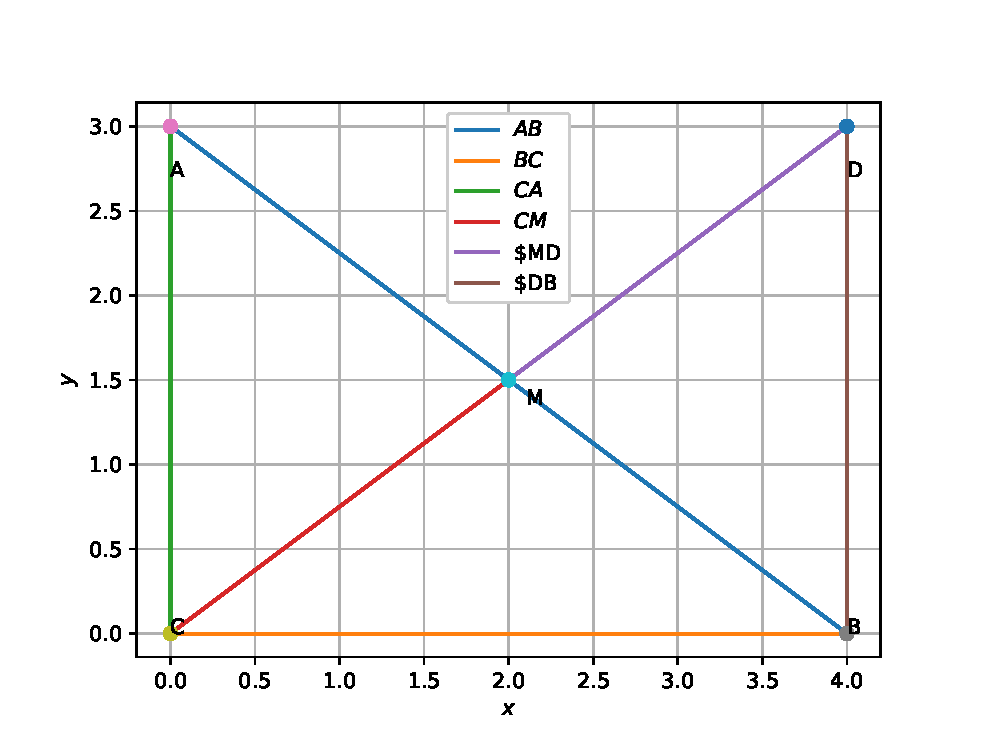
\includegraphics[width=\columnwidth]{./figs/triangle.eps}
\caption{Triangle generated using python}
\label{fig:tri_sss_py}
\end{figure}

%
and the equivalent latex-tikz code generating Fig. \ref{fig:tri_right_angle} is 
\begin{lstlisting}
figs/triangle.tex
\end{lstlisting}
%
The above latex code can be compiled as a standalone document as
\begin{lstlisting}
figs/triangle_fig.tex
\end{lstlisting}

%

%

%
%

\end{enumerate}

\section*{\textbf{Solution}}

From the figure, lets assume $\vec{C}$ to be the origin.
\newline
\begin{figure}[H]


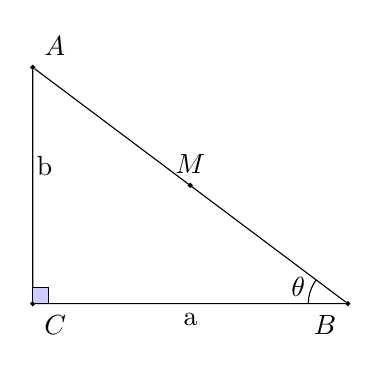
\begin{tikzpicture}
[scale=1,>=stealth,point/.style={draw,circle,fill = black,inner sep=0.5pt},]

%Triangle sides
\def\a{4}
\def\b{3}
\def\c{sqrt(\a^2+\c^2)}



%Labeling points
\node (A) at (0,\b)[point,label=above right:$A$] {};
\node (B) at (\a, 0)[point,label=below left:$B$] {};
\node (C) at (0, 0)[point,label=below right:$C$] {};
\node (M) at (\a*0.5,\b*0.5)[point,label=above:$M$] {};
%\node (D) at (\a,\b)[point,label=above right:$D$] {};


%Drawing triangle ABC
\draw (A) -- node[left] {$\textrm{}$} (B) -- node[below] {$\textrm{a}$} (C) -- node[above,xshift=1.5mm] {$\textrm{b}$} (A);

%Joining CD
%\draw (C)--(D);
%Joining BD
%\draw (B)--(D);

%Drawing and marking angles
%\tkzMarkAngle[fill=orange!40,size=0.5cm,mark=](A,M,C)
%\tkzMarkAngle[fill=orange!40,size=0.5cm,mark=](B,M,D)
\tkzMarkAngle[fill=green!40,size=0.5cm,mark=](A,B,C)
\tkzMarkRightAngle[fill=blue!20,size=.2](A,C,B)
%\tkzMarkRightAngle[fill=blue!20,size=.2](D,B,C)
%\tkzLabelAngle[pos=0.65](A,M,C){$\theta$}
%\tkzLabelAngle[pos=0.65](B,M,D){$\theta$}
\tkzLabelAngle[pos=0.65](A,B,C){$\theta$}


\end{tikzpicture}


\caption{$\triangle ACB$}
\end{figure}
$\vec{C}=0$
\newline
$\vec{CA}=b\hat{j}$
\newline
$\vec{CB}=a\hat{i}$
\newline
$\vec{M}$ is the position vector of mid-point of $\vec{BA}$.
\newline
$\vec{CM} = \vec{CB}+\vec{BM}$ [$\vec{BM}=(1/2)*\vec{BA}$]
\newline
$\vec{CM} = a\hat{i}+(1/2)(b\hat{j}-a\hat{i})$
\newline
Therefore, $\vec{CM}=(1/2)(b\hat{j}+a\hat{i})$
\newline
\begin{figure}[H]

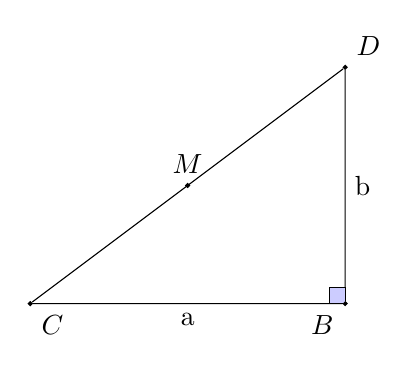
\begin{tikzpicture}
[scale=1,>=stealth,point/.style={draw,circle,fill = black,inner sep=0.5pt},]

%Triangle sides
\def\a{4}
\def\b{3}
\def\c{sqrt(\a^2+\c^2)}



%Labeling points
%\node (A) at (0,\b)[point,label=above right:$A$] {};
\node (B) at (\a, 0)[point,label=below left:$B$] {};
\node (C) at (0, 0)[point,label=below right:$C$] {};
\node (M) at (\a*0.5,\b*0.5)[point,label=above:$M$] {};
\node (D) at (\a,\b)[point,label=above right:$D$] {};


%Drawing triangle DBC
\draw (D) -- node[right] {$\textrm{b}$} (B) -- node[below] {$\textrm{a}$} (C) -- node[above,xshift=5mm] {$\textrm{}$} (D);

%Joining CD
%\draw (C)--(D);
%Joining BD
%\draw (B)--(D);

%Drawing and marking angles
%\tkzMarkAngle[fill=orange!40,size=0.5cm,mark=](A,M,C)
%\tkzMarkAngle[fill=orange!40,size=0.5cm,mark=](B,M,D)
%\tkzMarkAngle[fill=green!40,size=0.5cm,mark=](A,B,C)
%\tkzMarkRightAngle[fill=blue!20,size=.2](A,C,B)
\tkzMarkRightAngle[fill=blue!20,size=.2](D,B,C)
%\tkzLabelAngle[pos=0.65](A,M,C){$\theta$}
%\tkzLabelAngle[pos=0.65](B,M,D){$\theta$}
%\tkzLabelAngle[pos=0.65](A,B,C){$\alpha$}


\end{tikzpicture}

\caption{$\triangle DBC$}
\end{figure}
From the figure, $\vec{CD}=2(\vec{CM})$
\newline
$\vec{CD}=a\hat{i}+b\hat{j}$

\subsection*{\textbf{Sol.a)}}

$\triangle AMC$ and $\triangle DMB$ are congruent to each other by SAS congruency.
\newline
(i) Side AM  is equal to the corresponding side BM  [As M is midpoint of AB]
\newline
(ii)Side CM of is equal to corresponding side DM [As M is midpoint of DC]
\newline
(iii)$\angle AMC$ = $\angle DMB$ [ Vertically Opposite Angles]
\subsection*{\textbf{Sol.b)}}
In $\triangle ACB$  $(\norm{\vec{BA}})^2= a^2+b^2$
Since $\angle ACB$ = 90$^{\circ}$[ Pythagorus theorem]
\newline
In $\triangle DBC$ 
$cos \angle DBC= [((a^2+b^2-(\norm{\vec{CD}})^2)/2ab)] $
With the given vector values we get norm of $(\norm{\vec{BA}})=(\norm{\vec{CD}})$
\newline
$cos\angle DBC =[((a^2+b^2-(\norm{\vec{CD}})^2)/2ab)]$
$cos\angle DBC$=0
\newline
Therefore, $\angle DBC$ is right angle


\subsection*{\textbf{Sol.c)}}
$\triangle ACB$ and $\triangle DCB$ are congruent to each other in SAS congruency.
(i)Both the triangles have a common base , a.
\newline
(ii)AC = DB by using distance formula
\newline
(iii)$\angle ACB$ = $\angle DBC$ = 90$^{\circ}$ [ From Solution b)]

\subsection*{\textbf{Sol.d)}}
Since $\vec{CM}$ is halfway of $\vec{CD}$
\newline
$\norm{\vec{CM}}=\norm{\vec{CD}}$
\newline
From Solution b) it is clear that $\norm{\vec{CD}}=\norm{\vec{BA}}$
\newline
Therefore $\norm{\vec{CM}}=\frac{1}{2}\norm{\vec{AB}}$
\\
Hence, proved.


\end{document}
